\documentclass[titlepage]{article}
\usepackage[style=nature]{biblatex}
\usepackage{graphicx}
\usepackage{authblk}
\usepackage{hyperref}

\begin{document}

\title{Removing nonlinear batch effects using adversarial deep neural networks}
\author[1]{Jonathan B. Dayton}
\author[1,2]{Stephen R. Piccolo}
\affil[1]{Department of Biology, Brigham Young University, Provo, UT 84602 USA}
\affil[2]{Department of Biomedical Informatics, University of Utah, Salt Lake City, UT 84108 USA}

\maketitle

\begin{abstract}
	The abstract text goes here.
\end{abstract}

\section{Background}
Here is the text of your introduction.

\subsection{Subsection Heading Here}
Write your subsection text here.

\begin{figure}
	\centering
	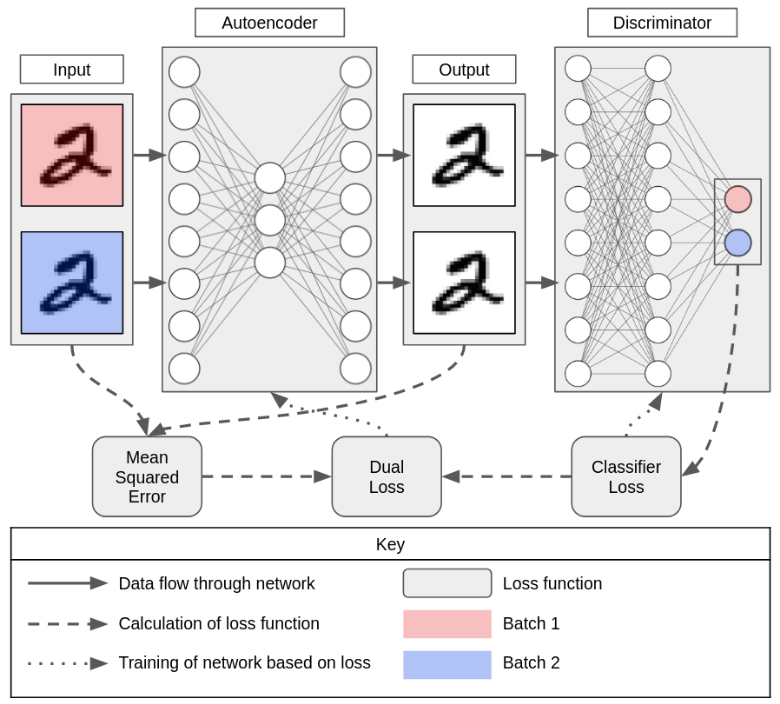
\includegraphics[width=4.5in]{figures/network}
	\caption{Network architecture}
	\label{simulationfigure}
\end{figure}

\section{Implementation}

\emph{\href{https://bmcbioinformatics.biomedcentral.com/submission-guidelines/preparing-your-manuscript/software-article}{Oxford Bioinformatics' guidelines} say that you should have an "Implementation" section instead of Materials and Methods.}

\begin{equation}
	\label{simple_equation}
	\alpha = \sqrt{ \beta }
\end{equation}

\section{Results}

\section{Discussion}

\section{Conclusions}

\end{document}
